\documentclass[12pt,
article,
type=bsc, %sta, diplom, bsc, pp, msc, dr, drfinal, sem, prosem
colorbacktitle,
instlogo,
accentcolor=tud1c,
twoside
]{tudthesis}

\usepackage[ngerman]{babel}
\usepackage[latin1]{inputenc}
\usepackage{url}
\usepackage{amsmath}
\usepackage{graphicx}
\usepackage{listings}
\usepackage{color} %red, green, blue, yellow, cyan, magenta, black, white
\usepackage{chngcntr}
\usepackage{pgfplots}
\usepackage{array}
\usepackage{amssymb}% http://ctan.org/pkg/amssymb
\usepackage{pifont}% http://ctan.org/pkg/pifont
\newcommand{\cmark}{\ding{51}}%
\newcommand{\xmark}{\ding{55}}%
\urlstyle{rm}

\newcommand{\getmydate}{%
\iflanguage{ngerman}{%
  \ifcase\month%
    \or Januar\or Februar\or M\"arz%
    \or April\or Mai\or Juni\or Juli%
    \or August\or September\or Oktober%
    \or November\or Dezember%
  \fi\ \number\year%
}%
\iflanguage{english}{%
  \ifcase\month%
    \or January\or February\or March%
    \or April\or May\or June\or July%
    \or August\or September\or October%
    \or November\or December%
  \fi\ \number\year%
}
}

\lstset{language=C++,
	belowcaptionskip=1\baselineskip,
	breaklines=true,
	frame=L,
	xleftmargin=\parindent,
	showstringspaces=false,
	basicstyle=\footnotesize\ttfamily,
	keywordstyle=\bfseries\color{green!40!black},
	commentstyle=\itshape\color{purple!40!black},
	identifierstyle=\color{blue},
	stringstyle=\color{orange},
}

\counterwithin{figure}{section} 
\counterwithin{table}{section} 

\setinstitutionlogo[height]{logo/ESlogo.png}

\setlength{\parindent}{0em}
\setlength{\parskip}{1em}

\begin{document}
	\counterwithin{lstlisting}{section}
	\thesistitle{Abschlussbericht Projektseminar Echtzeitsysteme}
	{Gruppe Crash Test Dummies}
	\author{Kai Cui, Feiyu Chang, Regis Fayard, Lars Semmler, David Botschek}
	
	\referee{Stefan Tomaszek}{Stefan Tomaszek}
	
	\iflanguage{english}{
		\department{	\mbox{Department of Electrical Engineering}\\ and Information Technology (FB18)\\\\Adjunct Member Department of\\ Computer Science (FB20)\\\\Prof. Dr. rer. nat. A. Sch�rr\\\ Merckstra�e 25\\64283 Darmstadt\\\\www.es.tu-darmstadt.de}
		\group{Real-Time Systems Lab}
	}{
		\department{Elektrotechnik und \\Informationstechnik (FB18)\\\\Zweitmitglied Informatik (FB20)\\\\Prof. Dr. rer. nat. A. Sch�rr\\\ Merckstra�e 25\\64283 Darmstadt\\\\www.es.tu-darmstadt.de}
		\group{Fachgebiet Echtzeitsysteme}
	}
	
	\dateofsubmit{\today}
	\makethesistitle
	\affidavit{Kai Cui, Feiyu Chang, Regis Fayard, Lars Semmler, David Botschek}
	
%	\cleardoublepage
%	\begin {abstract}
%	...
%	\end{abstract} 
	
	\cleardoublepage
	\pagenumbering{roman}
	\addtocontents{Anhang}{}
	\tableofcontents
	\clearpage
%	\listoffigures
%	\clearpage
%	\listoftables
%	\clearpage
	
	\pagenumbering{arabic}
	\section{Einf�hrung}
\label{sec:intro}

In der Automobilindustrie wird immer mehr auf autonomes Fahren gesetzt. Hier werden in der Entwicklung st�ndig neue Meilensteine erreicht, sodass ein Fahren ohne eine Person am Steuer immer realistischer wird.

Eine kleine Einf�hrung will hier das Projektseminar Echtzeitsysteme der TU Darmstadt bieten. Anhand eines Modellautos werden Ans�tze realit�tsnaher Algorithmen diskutiert und ausprobiert. Die Kommunikation mit dem Auto geschieht mit Hilfe des Programms Robot Operating System (ROS). Mit dieser Methode testet auch der Kooperationspartner \glqq Fachgebiet Fahrzeugtechnik (FZD)\grqq{} L�sungen am echten Auto, was die Relevanz dieses Projektseminars unterstreicht.

Ein weiterer, nicht weniger wichtiger Schwerpunkt des Seminars ist die erfolgreiche Planung und Durchf�hrung der Gruppenarbeit. Die 5 Mitglieder der einzelnen Gruppen werden aus verschiedenen Vertiefungsrichtungen zugeteilt, damit jeder eigenes Knowhow mitbringen kann. Die verschiedenen Rollen und Verantwortlichkeiten werden im Team erprobt.

\paragraph{Fahrzeug}
Dem Fahrzeug stehen verschiedene Sensoren wie der Ultraschall-, Gyro-, und Hallsensor sowie eine Kinect-Kamera zur Verf�gung um das Umfeld m�glichst realit�tsnah wahrzunehmen. Durch die Kamera kann man sowohl auf ein Farbbild als auch auf ein Tiefenbild zugreifen was eine pr�zise Bildverarbeitung erm�glicht.

\paragraph{Aufgaben}
Die verschiedenen Fortschritte wurden nach einzelnen Aufgaben gestaffelt. Das Abfahren eines Rundkurses anhand der Analyse zweier Linien stellte die Basis- und Pflichtaufgabe dar. Weitere Aufgaben durften selbst vorgeschlagen werden, als m�gliche Beispiele wurden Spurwechsel, Hinderniserkennung und Verkehrsschilderkennung vorgeschlagen.
Unsere Gruppe entschied sich f�r Spurwechsel und Erkennung der Schilder.
Zum Projektumfang z�hlten aber genauso auch das Festlegen von und Pr�fen in Testszenarien um die Funktionalit�t und Zuverl�ssigkeit autonomer Ste�rungen sicherzustellen.  

	\clearpage
	\section{Projektorganisation}
F�r einen reibungslosen Ablauf haben wir zu Beginn geplant, wie wir unsere Kommunikation gestalten, und konnten mit Hilfe der unten aufgef�hrten Tools eine erfolgsversprechende Roadmap erzielen.

Die Seminarorganisation schrieb ein regelm��iges Treffen mit dem Seminarleiter vor um Hilfestellungen und Tipps zu erm�glichen. Vom Fachgebiet Fahrzeugtechnik wurde alle zwei Wochen eine Fragerunde zu regelungstechnischen Problemen angeboten. Dieses Treffen diente auch als Austausch mit den anderen Gruppen.

In unsere Kleingruppe entschieden wir uns dazu, uns einmal w�chentlich zusammen am Auto zu treffen um gegenseitiges Helfen zu erm�glichen und den n�chsten kurzen Abschnitt zu planen.

Den Rest der Woche wurde selbstst�ndig an den neu zugeteilten Aufgaben weitergearbeitet.
Bei akuten Fragen und Problemen fand ebenso eine st�ndige Kommunikation �ber WhatsApp statt.

\subparagraph{Trello}
Damit wir die Aufgaben pr�zise und strukturiert festhalten konnten haben wir uns f�r das Organisations-Tool Trello entschieden. Hiermit konnten wir durch Anlegen von Listen unsere Punkte in \glqq ToDo\grqq, \glqq Meeting\grqq, \glqq Gemacht\grqq{} und \glqq Aufgaben f�r die Zukunft\grqq{} aufteilen.

\subparagraph{Github}
F�r die Synchronisierung des Programmcodes haben wir das Versionsverwaltungsprogramm git genutzt. Dadurch konnten wir komfortabel den Programmiercode des Fahrzeugs austauschen sowie bei Fehlern auf alte Code-Zust�nde zur�ckgreifen.

Ebenso konnten wir beim Programmieren auf eine Reihe vorhandener Bibliotheken und Funktionen zur�ckgreifen. 

\subparagraph{OpenCV}
Mit OpenCV \cite{OpenCV} konnten wir die Bilder verarbeiten und die ben�tigten Informationen herausfiltern. Auch der Algorithmus zur Bilderkennung basiert auf einem Beispiel einer OpenCV-Demo \cite{findObject}

\subparagraph{quadprog++}
Die Bibliothek quadprog++ \cite{quadprog} stellt eine Funktion bereit, welche die Optimierung des Optimierungsproblems der modellpr�diktiven Regelung erleichtert.

Auch haben wir mit dem Programm doxygen \cite{doxygen} und dem darauf basierenden rosdoc\_lite eine �bersichtliche Dokumentation unseres Codes mit Kommentaren erstellt.
	\clearpage
	\section{Protokoll}
	\begin{table}[h]
		\renewcommand{\arraystretch}{1.5}
		\begin{center}
		\begin{tabular}{|>{\centering\arraybackslash}p{0.7\textwidth}|>{\centering\arraybackslash}p{0.06\textwidth}|>{\centering\arraybackslash}p{0.06\textwidth}|>{\centering\arraybackslash}p{0.06\textwidth}|}
			\hline
			Testfall& 14.2. & 21.2. & 28.2. \tabularnewline
			\hline
			Das Fahrzeug f�hrt rechts und links herum autonom ohne die Fahrbahnbegrenzung zu ber�hren.& \xmark &\checkmark &\checkmark \tabularnewline
			\hline
			Das Fahrzeug f�hrt auf einer Fahrspur autonom ohne die Spur zu verlassen. & \checkmark & \checkmark & \checkmark \tabularnewline
			\hline
			Das Fahrzeug f�hrt eine Runde unter 30s.& \checkmark \newline $25s$ & \checkmark \newline $19s$ & \checkmark \newline $19s$ \tabularnewline
			\hline
			Das Fahrzeug kommt von der Fahrbahn ab und muss daraufhin anhalten.& \xmark & \xmark & \checkmark \tabularnewline
			\hline
			Das Fahrzeug startet mittig auf der Fahrbahn im {45} Winkel zur Fahrbahnbegrenzung & \checkmark & \checkmark & \checkmark  \tabularnewline
			\hline
			Das Fahrzeug startet mittig auf der Fahrbahn im {60} Winkel zur Fahrbahnbegrenzung& \xmark & \checkmark & \checkmark \tabularnewline
			\hline
			Bei einem Stoppschild h�lt das Fahrzeug f�r 3s an und f�hrt danach weiter.& \xmark & \checkmark & \checkmark \tabularnewline
			\hline
			Bei einem Geschwindigkeitsschild f�hrt das Fahrzeug ab dem Schild mit verringerter Geschwindigkeit weiter.& \xmark & \checkmark & \checkmark \tabularnewline
			\hline
			Bei einem Fahrbahnverengung Schild wechselt das Fahrzeug 
			die Fahrspur.& \xmark & \checkmark & \checkmark \tabularnewline
			\hline
			Schilderkennung und autonomes Fahren muss gleichzeitig ohne wahrnehmbare Beeintr�chtigung funktionieren.& \xmark & \xmark & \checkmark \tabularnewline
			\hline
			
		\end{tabular}
		\end{center}
	\end{table}
	\clearpage
	\section{Regelans{�}tze}
  
\subsection{1.Ansatz}
  
\clearpage
\subsection{Modellpr�diktiver Regelungansatz}
Ein zweiter experimenteller Ansatz, der im Rahmen des Projektseminars verfolgt wurde, ist die sogenannte lineare modellpr�diktive Regelung. Bei dieser wird anhand eines linearen, diskretisierten Fahrzeugmodells �ber ein quadratisches Optimierungsproblem eine L�sung f�r die optimalen Lenkwinkel berechnet. Diese sind optimal in dem Sinne, dass eine Linearkombination der mittleren quadratischen Abweichungen des pr�diktierten Systemzustands und Stellgr��e zu einer vorgegebenen Solltrajektorie �ber einen endlichen Zeithorizont hinaus minimiert wird.

Ein gro�er Vorteil dieses Verfahrens ist, dass es automatisch Stellgr��enbeschr�nkungen beachtet und es somit nicht zu Pr�diktionsfehlern durch unbeschr�nkte Stellgr��en kommt. Durch die Methode erh�lt man zugleich den gesamten Stellgr��enverlauf f�r den eingestellten Zeithorizont, sodass es au�erdem m�glich ist, �ber l�ngere Zeit ohne Neuberechnung an einer Solltrajektorie entlang zu fahren, vorausgesetzt das linearisierte Modell ist f�r die gegebene Zustandstrajektorie ausreichend genau. 

Zun�chst bringen wir das Problem in die Form, die f�r die lineare modellpr�diktive Regelung ben�tigt wird. Dabei orientieren wir uns an \cite{hovd2004brief} sowie an Vorarbeiten von Herrn Eric Lenz am FG RTM. Wir gehen aus vom Querf�hrungsmodell in Gleichung \ref{eq:quer} von Herrn Eric Lenz am FG RTM, welches bereits das Ackermannmodell auf eine Raumdimension reduziert:
\begin{align}
	\label{eq:quer}	
	\begin{pmatrix} \dot{y} \\ \dot{\varphi_K} \end{pmatrix}
	= 
	\begin{pmatrix} 0 & v \\ 0 & 0 \end{pmatrix}
	\begin{pmatrix} {y} \\ {\varphi_K} \end{pmatrix}
	+ 
	\begin{pmatrix} v\cdot \frac{l_H}{l} \\ \frac{v}{l} \end{pmatrix}
	\varphi_L^*
	= \mathbf{Ax + Bu}
\end{align}
Das Modell wird per Hand mit der Abtastperiode $T$ diskretisiert zu
\begin{align}
	\mathbf{A_d} = e^{\mathbf{A}T} = 
	\begin{pmatrix} 1 & vT \\ 0 & 1 \end{pmatrix} \\
	\mathbf{B_d} = \int_0^T e^{\mathbf{A}\tau} \mathbf{B} d\tau = 
	\begin{pmatrix} \frac{vTl_h}{l} + \frac{v^2T^2}{2l} \\ \frac{vT}{l} \end{pmatrix} \\	
	\begin{pmatrix} y(k+1) \\ \varphi_K(k+1) \end{pmatrix}
	= 
	\begin{pmatrix} 1 & vT \\ 0 & 1 \end{pmatrix} 
	\begin{pmatrix} y(k) \\ \varphi_K(k) \end{pmatrix}
	+ 
	\begin{pmatrix} \frac{vTl_h}{l} + \frac{v^2T^2}{2l} \\ \frac{vT}{l} \end{pmatrix} 
	\varphi_L^*(k)
	\label{eq:diskret}	
\end{align}
Es sei nun eine Trajektorie nach den Gleichungen \ref{eq:traj1}, \ref{eq:traj2} gegeben, deren Erzeugung wir an sp�terer Stelle erl�utern.
\begin{align}	
	\label{eq:traj1}
	x_{ref} &= 
	\begin{pmatrix} x_{ref,1} & x_{ref,2} & \hdots & x_{ref,n-1} & x_{ref,n} \end{pmatrix}^T \\ 
	\label{eq:traj2}
	u_{ref} &= 
	\begin{pmatrix} u_{ref,0} & u_{ref,1} & \hdots & u_{ref,n-2} & u_{ref,n-1} \end{pmatrix}^T 
\end{align}
Dann definieren wir
\begin{align}
	\hat{Q} &= 100 \cdot diag(1,0,\cdots,1,0) ;\quad
	\hat{P} = \mathbf{I}_{n,n} ;\quad
	-U_{min} = U_{max} = 21^o \nonumber\\
	x_0 &= 
	\begin{pmatrix} y(k) \\ 0 \end{pmatrix} ;\quad
	A = 
	\begin{pmatrix} 1 & vT \\ 0 & 1 \end{pmatrix} ;\quad
	B = 
	\begin{pmatrix} \frac{vTl_h}{l} + \frac{v^2T^2}{2l} \\ \frac{vT}{l} \end{pmatrix} \nonumber\\
	\chi_0 &= 
	\begin{pmatrix} A \\ A^2 \\ \vdots \\ A^{n-1} \\ A^n \end{pmatrix}
	x_0
	+
	\begin{pmatrix} 
		B & 0 & \hdots & 0 & 0 \\ 
		AB & B & \ddots & \vdots & \vdots \\ 
		\vdots & \vdots & \ddots & 0 & 0 \\ 
		A^{n-2}B & A^{n-3}B & \hdots & B & 0 \\ 
		A^{n-1}B & A^{n-2}B & \hdots & AB & B
	\end{pmatrix}
	u_{ref} - x_{ref} 
\end{align}
Wir k�nnen dann das folgende quadratische Optimierungsproblem f�r $n$ Zeitschritte definieren \cite{hovd2004brief}, welches die quadratischen Positionsabweichungen �ber $n$ Zeitschritte vorw�rts minimiert.
\begin{align}
	\min_v f(v) 
	&= \min_v 0.5v^T\tilde{H}v + c^Tv \\
	&= \min_v (x_0 - x_{ref,0})^TQ(x_0 - x_{ref,0}) + \chi_0^T\hat{Q}\chi_0 + 2\chi_0^T\hat{Q}\chi_v + \chi_v^T\hat{Q}\chi_v + v^T\hat{P}v 
\end{align}
mit den Stellgr��en-Nebenbedingungen
\begin{align}
	\mathbf{I}_{n,n}v &\geq \begin{pmatrix} U_{min} \\ \vdots \\ U_{min} \end{pmatrix} - u_{ref} \\
	-\mathbf{I}_{n,n}v &\geq -\begin{pmatrix} U_{max} \\ \vdots \\ U_{max} \end{pmatrix} + u_{ref}
\end{align}
Da wir keine Zustandsgr��enbeschr�nkung vorsehen, ben�tigen wir die restlichen Nebenbedingungen aus \cite{hovd2004brief} nicht. Dieses Optimierungsproblem wird f�r die gegebene Trajektorie on-line auf dem Fahrzeug gel�st, und der folgende optimale Stellgr��enverlauf wird abgespielt:
\begin{align}
	\varphi_{L,i} = \arctan(\varphi_{L,i}^*) = \arctan(u_i) = \arctan(v_i + u_{ref,i})
\end{align} 
Die Konvergenz, Optimalit�t und numerische Stabilit�t der L�sung des Optimierungsproblems der linearen modellpr�diktiven Regelung ist hierbei durch die Verwendung von Methoden aus der quadratischen Programmierung, z.B. hier \cite{goldfarb1983numerically}, sichergestellt.

Wir haben hier die Gewichtungsmatrizen $\hat{Q}, \hat{P}$ so gesetzt, dass n�herungsweise lediglich die Positionsabweichung zur Solltrajektorie minimiert werden soll. Dies erlaubt es uns daher, als Solltrajektorie den Sollstellgr��enverlauf zu ignorieren und eine beliebige Sollwinkeltrajektorie vorzugeben, da Inkonsistenzen mit dem Sollzustandsverlauf kaum ins Gewicht fallen:
\begin{align}	
u_{ref} &= 
\begin{pmatrix} 0 & 0 & \hdots & 0 & 0 \end{pmatrix}^T 
\end{align}
Als n�chstes wird die Beschaffung der Sollzustandstrajektorie erl�utert. Dazu bedienen wir uns der Kamera, dessen Farbdaten zun�chst mithilfe einer inversen Perspektiventransformation (IPM) auf ein Birdeye-View gebracht werden. Beispielhaft ist ein bearbeitetes, transformiertes Bild in Abbildung \ref{fig:quadratic} zu sehen.

Das Bild wird in horizontale Streifen einer vordefinierten Breite unterteilt. Anschlie�end werden die Streifen nach den Fahrbahnbegrenzungsfarben gefiltert und Spaltenhistogramme gebildet. Die Histogrammmaxima am n�chsten zur Mitte des Bildes mit einem vordefinierten Mindestabstand werden selektiert. In diesem Fall also bis zu zwei Seitenstreifenpunkte und bis zu ein Mittellinienpunkt. Diese sind in Abbildung \ref{fig:quadraticorig} als schwarze Kreise eingezeichnet.

Anschlie�end werden diese Punkte verwendet, um sinnvolle Wegpunkte zu definieren. Diese sind in der Abbildung \ref{fig:quadraticorig} als gr�ne Kreise eingezeichnet. Wegpunkte werden priorisiert zwischen einen Mittellinienpunkt und den Seitenstreifenpunkt der entsprechenden Fahrbahnseite gelegt. Falls das nicht m�glich ist, z.B. weil einer der Punkte nicht existiert, legen wir ihn $\frac{1}{4}$ oder $\frac{3}{4}$ zwischen die Seitenstreifenpunkte je nach Fahrbahnseite. Falls auch das nicht m�glich ist, k�nnen zus�tzliche Punkte aus den bereits existierenden inferiert werden, falls mindestens ein Seitenstreifenpunkt existiert.

\begin{figure}[ht]
	\centering
	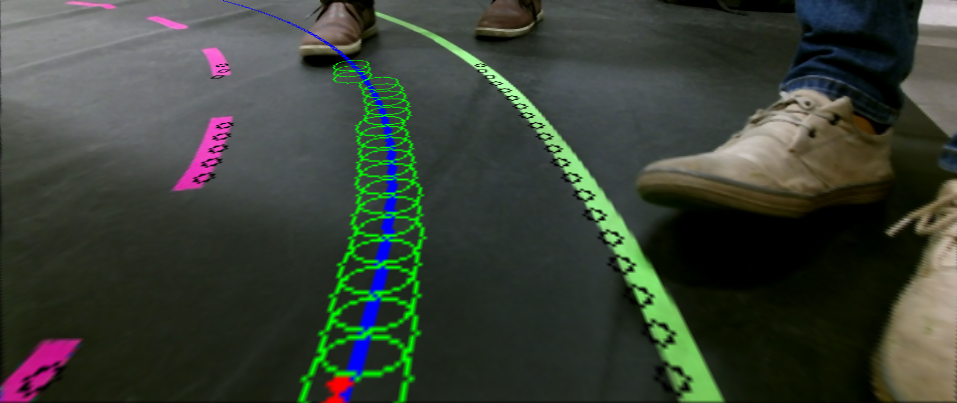
\includegraphics[width=0.9\textwidth]{pics/windowedorig.png}
	\caption{Bearbeitetes, r�cktransformiertes Bild mit quadratischer Trajektorie. Sichtbar sind Wegpunkte (gr�ne Kreise), die Solltrajektorie (blaue Linie), die pr�diktierte Trajektorie (rote Punkte) und Lanepunkte (schwarze Kreise)}
	\label{fig:quadraticorig}
\end{figure}

Mithilfe dieser Wegpunkte kann man nun eine Trajektorie $x_{ref}$ erzeugen.In Abbildung \ref{fig:quadraticorig} ist die blaue Linie eine quadratische Trajektorie, die an die gr�nen Wegpunkte gefittet wird. Die Trajektorie scheint zun�chst gut an die Fahrbahn angepasst zu sein. Man erkennt, dass die Solltrajektorie nicht einhaltbar ist, da die Querabweichung sich aus dem Unterschied zwischen polynomiell extrapolierter Solltrajektorie und Roboterposition zusammensetzt und nicht bei null beginnt. Dies ist kein Problem, da lediglich der quadratische Fehler �ber die n�chsten Zeitschritte minimiert wird. 

\begin{figure}[ht]
	\centering
	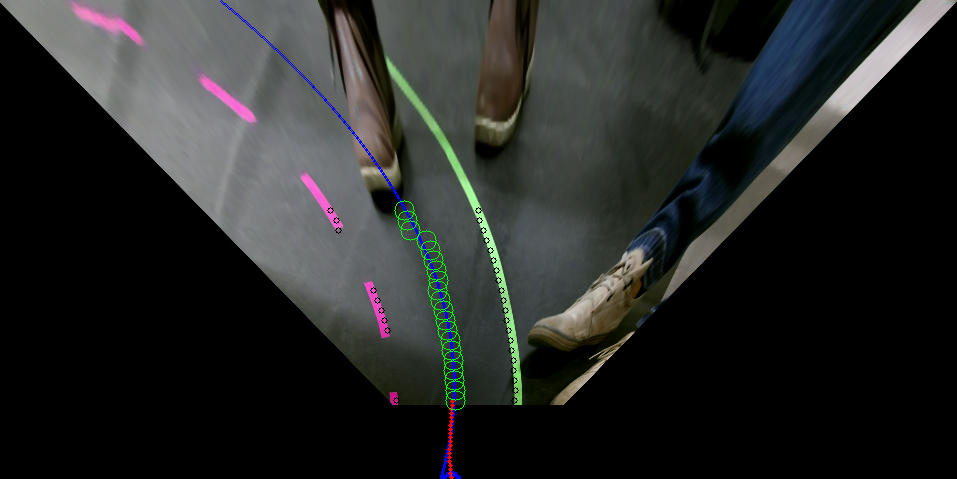
\includegraphics[width=0.9\textwidth]{pics/windowed.png}
	\caption{Transformierte und um Roboterposition erweiterte Version von Abbildung \ref{fig:quadraticorig}.}
	\label{fig:quadratic}
\end{figure}

Ein Problem l�sst sich in Abbildung \ref{fig:quadratic} jedoch feststellen: Die Trajektorien sind aufgrund der polynomiellen Extrapolation nicht station�r und sehr variant. Zus�tzlich kommt hinzu, dass die Regressionsmethode nicht rotationsinvariant ist, denn eine Rotation der Wegpunkte f�hrt aufgrund der vertikalen Polynomausrichtung zu einer v�llig anderen Trajektorie. Diese Umst�nde f�hren dazu, dass die Regelung versagt.

Eine andere einfache L�sung ist es, nicht zu interpolieren, sondern wie in Abbildung \ref{fig:direct} zu sehen eine direkte lineare Trajektorie zum n�chstliegenden Wegpunkt zu setzen. Dadurch wird die Trajektorie deutlich robuster und die Regelung funktioniert wie erwartet. Dasselbe Problem hat man jedoch im begrenzten Ma�e auch f�r die direkte lineare Trajektorie. Selbst wenn man auf Extrapolation verzichtet und ausreichend Mittelung verwendet, ist der unterste Bildpunkt aufgrund der auftretenden Rotation des gegen�ber der Roboterposition orthogonal ausgerichteten Bildes geringf�gig variant. Zus�tzlich kann es durch die Diskretisierung bei zu gro�en Zeitschritten zu �berschwingen trotz Einhaltung der diskreten Zustandssollwerte kommen.

\begin{figure}[ht]
	\centering
	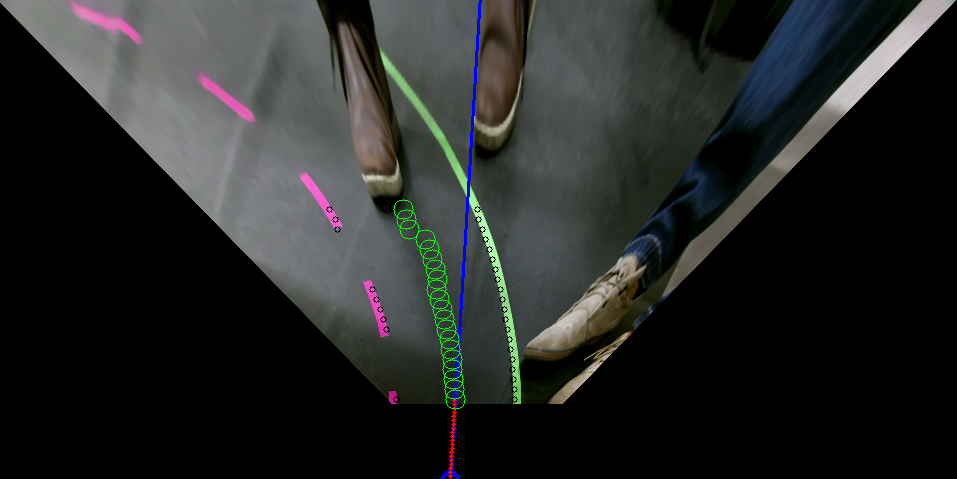
\includegraphics[width=0.9\textwidth]{pics/windoweddirect.png}
	\caption{Bearbeitetes, untransformiertes Bild mit quadratischer Trajektorie. Sichtbar sind Wegpunkte (gr�ne Kreise), die Solltrajektorie (blaue Linie), die pr�diktierte Trajektorie (rote Punkte), Lanepunkte (schwarze Kreise) und die Roboterposition relativ zum Bild (Anfangspunkt der pr�diktierten Trajektorie, gro�er blauer Kreis)}
	\label{fig:direct}
\end{figure}

Mit dieser Bildtrajektorie und den Bildtransformationsparametern lassen sich dann diskrete Trajektoriensollwerte $x_{ref,i}$ erzeugen, indem das kinematische Querf�hrungsmodell angenommen wird: F�r jeden Trajektorienzeitschritt wird eine konstante Vorw�rtsbewegung abh�ngig von der Geschwindigkeit ausgef�hrt, um den n�chsten Positionssollwert zu ermitteln.

Das gr��te Problem sind die Nichtlinearit�ten. Dieser Ansatz erlaubt noch weitere Verbesserungen, um besseres Regelverhalten zu erreichen und insbesondere hohe Geschwindigkeiten ausreichend genau zu regeln. Darauf wird in diesem Projektseminar aber aufgrund der abweichenden Zielsetzung verzichtet.

Es bietet sich zuk�nftig an, das Fahrzeugmodell durch ein nichtlineares Modell zu ersetzen. Damit landet man bei der nichtlinearen modelpr�diktiven Regelung (NMPC), z.B. \cite{allgower2012nonlinear}, bei der aufgrund der nichtlinearen Nebenbedingungen die Konvergenz zum Optimum zwar zun�chst nicht formal sichergestellt ist, aber praktisch gesehen klappt. 

Schlie�lich k�nnte man auch die Trajektoriengenerierung �berarbeiten. Eine naheliegende Wahl, um auch mit Bildraten von unter 1 Hz auszukommen, ist die Verwendung der direkten Trajektorie bis zum ersten Wegpunkt und darauffolgende Verwendung der quadratischen Trajektorie. Da die quadratische Trajektorie in diesem Fall nicht mehr extrapoliert, bietet diese eine hervorragende Trajektorienform f�r eine Regelung mit wenigen Bildern. 
	\clearpage
	\section{Schilderkennung}
Als Vertiefungsaufgabe haben wir uns entschieden, eine Schilderkennung zu implementieren. Unser Ziel beschr�nkt sich darauf, drei verschiedene Schilder zu erkennen, auf die das Auto dann reagiert. Diese Schilder sind in Abbildung \ref{fig:v1} abgebildet. Im Folgenden werden die zwei Ans�tze erkl�rt, die wir f�r die Realisierung verfolgt haben.

\begin{figure}[ht]
	\centering
	
\includegraphics[width=0.25\textwidth]{pics/Stopschild.png}
	
\includegraphics[width=0.25\textwidth]{pics/spurwechselschild.jpg}
	
\includegraphics[width=0.25\textwidth]{pics/Geschwindikeitsschild.png}
	\caption{Verwendete Schilder. Links: Auf H�he des Schildes 2 s anhalten. Mitte: Auf die andere Spur wechseln. Rechts: Geschwindigkeit verringern auf 1 km/h f�r 10 s}
	\label{fig:v1}
\end{figure}

\subsection{Erster Ansatz: Find-Object}
Unser erster Ansatz f�r die Schilderkennung war es, das ROS-Packet Find-Object von IntRoLab \cite{findObject} zu benutzen. Dieses erm�glicht es, mit einer grafischen Benutzeroberfl�che (siehe Abbildung \ref{fig:v2}), Referenzbilder zu laden, welche im Live-Bild der Kamera gesucht werden. Verschiedenen Suchalgorithmen (SIFT, SURF, FAST, BRIEF etc.) und Parameter konnten f�r schnelles Prototyping ausprobiert werden. 

\begin{figure}[ht]
	\centering
	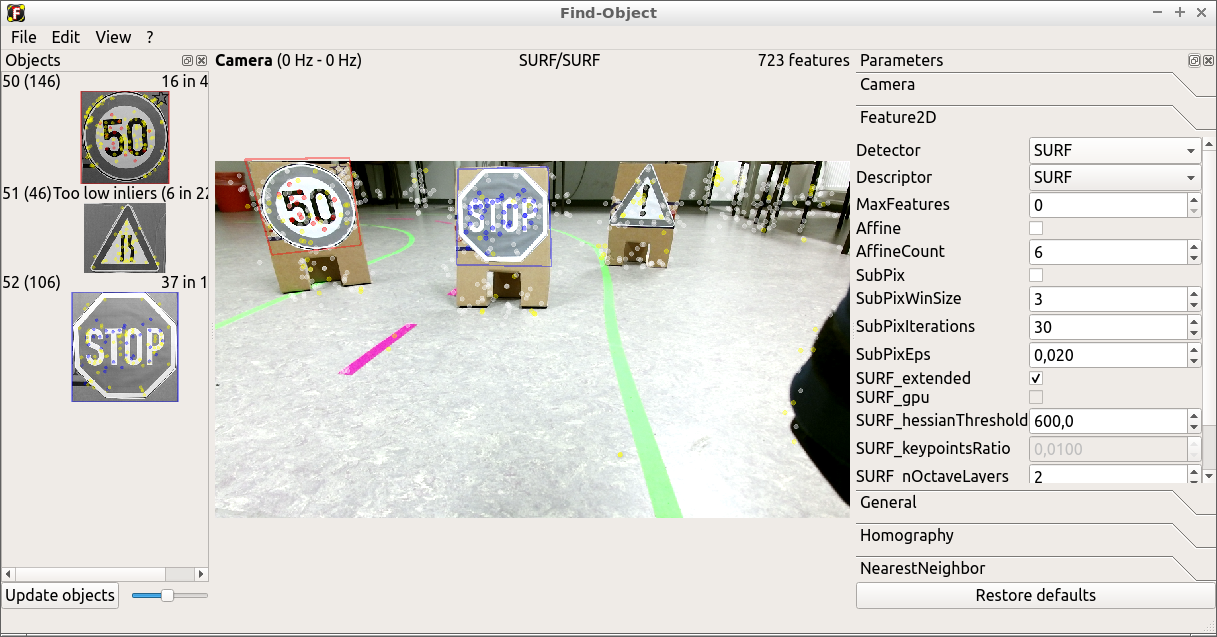
\includegraphics[width=0.9\textwidth]{pics/find_object_sceenshot.png}
	\caption{Grafische Benutzeroberfl�che von Find-Object. Links: Referenzbilder. Mitte: Kamerabild. Rechts: Parameter.}
	\label{fig:v2}
\end{figure}

\subparagraph{Probleme mit diesem Ansatz}
Als wir die Schilderkennung und den Regler f�r die Steuerung gleichzeitig laufen lie�en, begann das Auto stark zu schwingen und es war diesem nicht mehr m�glich die Spur korrekt zu halten. Die Performanz-Probleme konnten wir auf die CPU zur�ckf�hren, welche alleine durch die Verwendung der Kinect-Kamera zu ca. 50 \% ausgelastet war. Au�erdem ist das Paket Find-Object mit seinen umfangreichen Funktionen (von denen wir nicht alle ben�tigten), sehr rechenintensiv. So musste ein anderer Ansatz mit einem simplen, �berschaubaren Codeumfang angewendet werden.

\subsection{Finaler Ansatz: Schilderkennung mit SURF}
Mit dem ersten Ansatz hatten wir experimentell ermittelt, dass der Suchalgorithmus SURF (Speeded Up Robust Features) \cite{bay2006surf} f�r unser Anwendungsszenario am schnellsten und robustesten funktioniert. Schilder werden unabh�ngig von Gr��e und Orientation erkannt.

Als Code-Basis haben wir bestehenden OpenCV-Beispielcode verwendet. Diesen haben wir f�r unsere Zwecke angepasst, damit dieser mit ROS und der Kinect-Kamera kompatibel ist, und haben Funktionen wie Multi-Objekt-Erkennung hinzugef�gt.

\begin{figure}[ht]
	\centering
	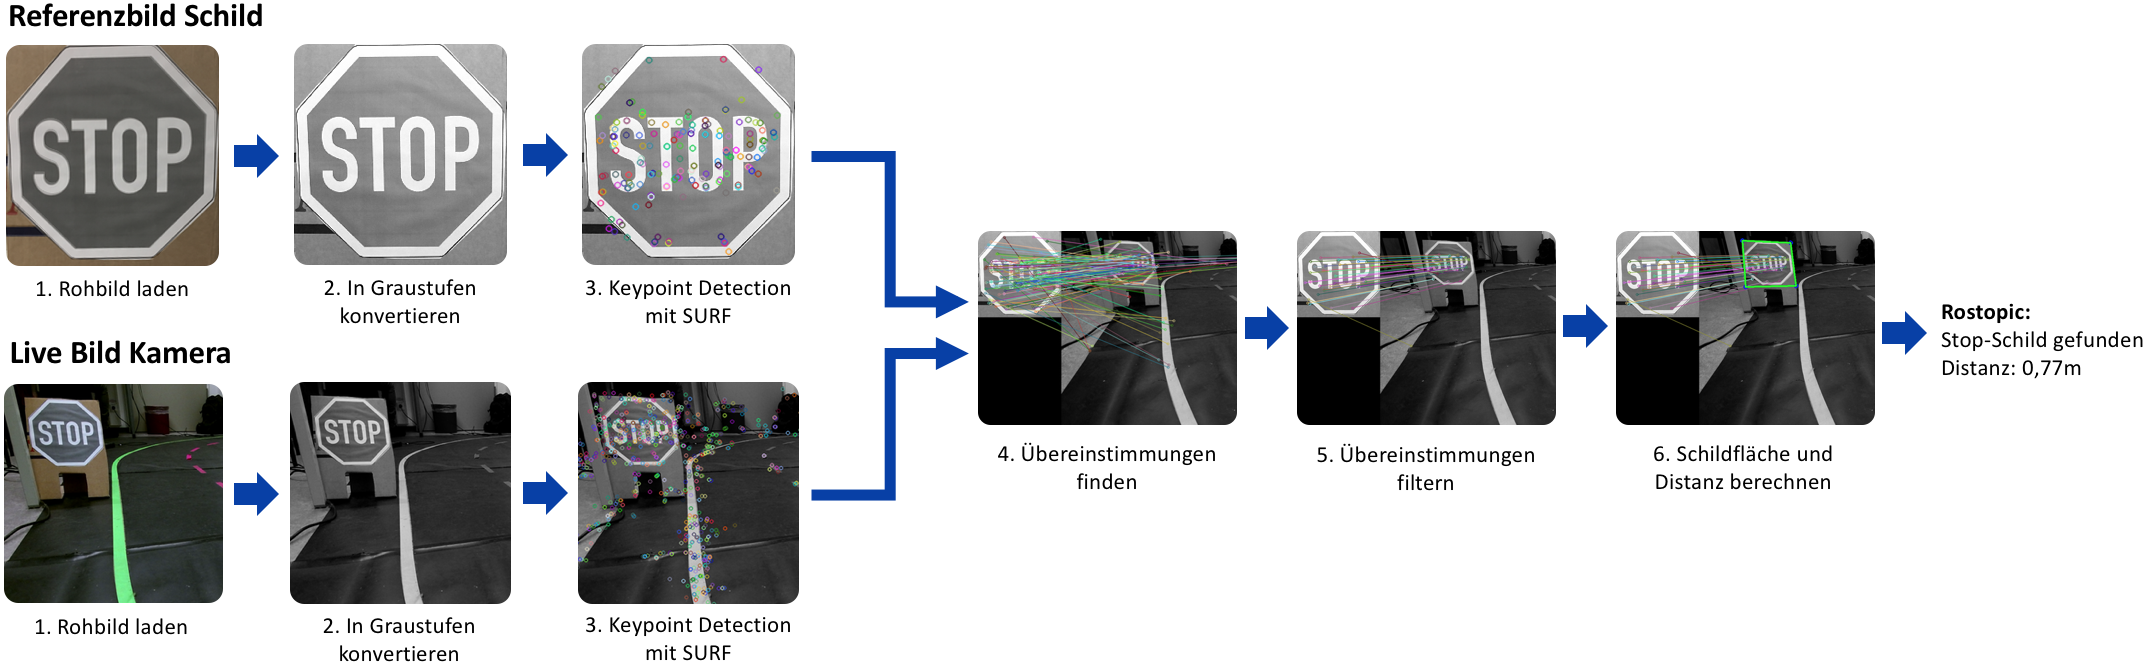
\includegraphics[width=0.9\textwidth]{pics/Schildererkennung-Pipeline.png}
	\caption{Schilderkennungs-Pipeline}
	\label{fig:v3}
\end{figure}

Um die Funktionsweise unseres Ansatzes zu erkl�ren, gehen wir die Schilderkennung-Pipeline Schritt f�r Schritt durch:

\subparagraph{Schritt 1}: Schild-Referenzbilder und das aktuellste Bild der Kamera werden geladen.

\subparagraph{Schritt 2}: Beide Bilder werden in Graustufen konvertiert, da Farbinformationen f�r diese Art der Objekterkennung irrelevant sind.

\subparagraph{Schritt 3}: Mit dem Detektor SURF wird in beiden Bildern separat nach markanten Punkten (auch Keypoint oder Point-of-Interest genannt) gesucht. Jeder Keypoint wird als ein Vektor von Eigenschaften (Koordinaten, Durchmesser, Winkel, Octave etc.) beschrieben.

\subparagraph{Schritt 4}: Nun wird nach �bereinstimmungen zwischen den Keypoints des Referenzbildes und des Kamerabildes gesucht. In diesem Schritt werden f�r jeden Keypoint des Referenzbildes zwei Keypoints aus dem Kamera-Bild gesucht, welche die gr��te Gemeinsamkeit haben. Daf�r wird der Nearest-Neighbor Algorithmus von FLANN (Fast Library for Approximate Nearest Neighbors) \cite{flann_pami_2014} genutzt.

\subparagraph{Schritt 5}: Anschlie�end werden die �bereinstimmungen gefiltert, so dass wir nur noch die besten �bereinstimmungen haben. Dazu verwenden wir den Lowe's-Ratio-Test \cite{lowe2004distinctive}, dieser schaut sich die Distanz zwischen dem Keypoint des Referenzbildes und dem des Kamerabild an und filtert �bereinstimmungen aus, welche den Vorgegebenen Threshold nicht erf�llen. Mit Distanz ist hier keine physikalische Distanz gemeint, sondern die Euklidische Distanz von zwei Keypoint-Vektoren. Dieser gibt den Wert der �hnlichkeit an.

\subparagraph{Schritt 6}: Wenn ein Schild gefunden wird, wird die physikalische Distanz vom Schild zum Auto ermittelt und diese wird auf einem ROS-Topic ausgegeben: \\
Wenn das Stoppschild erkannt wird: /sign\_detection\_node/StopSign \\
Wenn das Geschwindigkeitsschild erkannt wird: /sign\_detection\_node/LaneSign \\
Wenn das Spurwechselschild erkannt wird: /sign\_detection\_node/SpeedSign 

\subparagraph{Distanz vom Auto zum Schild ermitteln}
Um die Distanz vom Auto zum Schild zu ermitteln, war unsere erste Idee, das Tiefenbild der Kinect zu nutzen. Dieses verbraucht aber zu viel Rechenleistung, sodass die Regelung nicht mehr richtig funktioniert.

Daher verwenden wir die Fl�che des gefundenen Bildes, um diese in eine Distanz umzurechnen. Daf�r haben wir f�r verschiedene Distanzen gemessen, wie gro� die Fl�che ist und haben mittels Regressionsanalyse nach einer Funktion gesucht, welche die Messpunkte m�glichst gut beschreibt. Wie in Abbildung \ref{fig:v4} zu sehen, werden die Messpunkte am besten von einer Potenzfunktion beschrieben:
 
\begin{align*}
	d = 385 * A^{-0.6385}
\end{align*}

\clearpage
\begin{figure}[h]
	\centering
	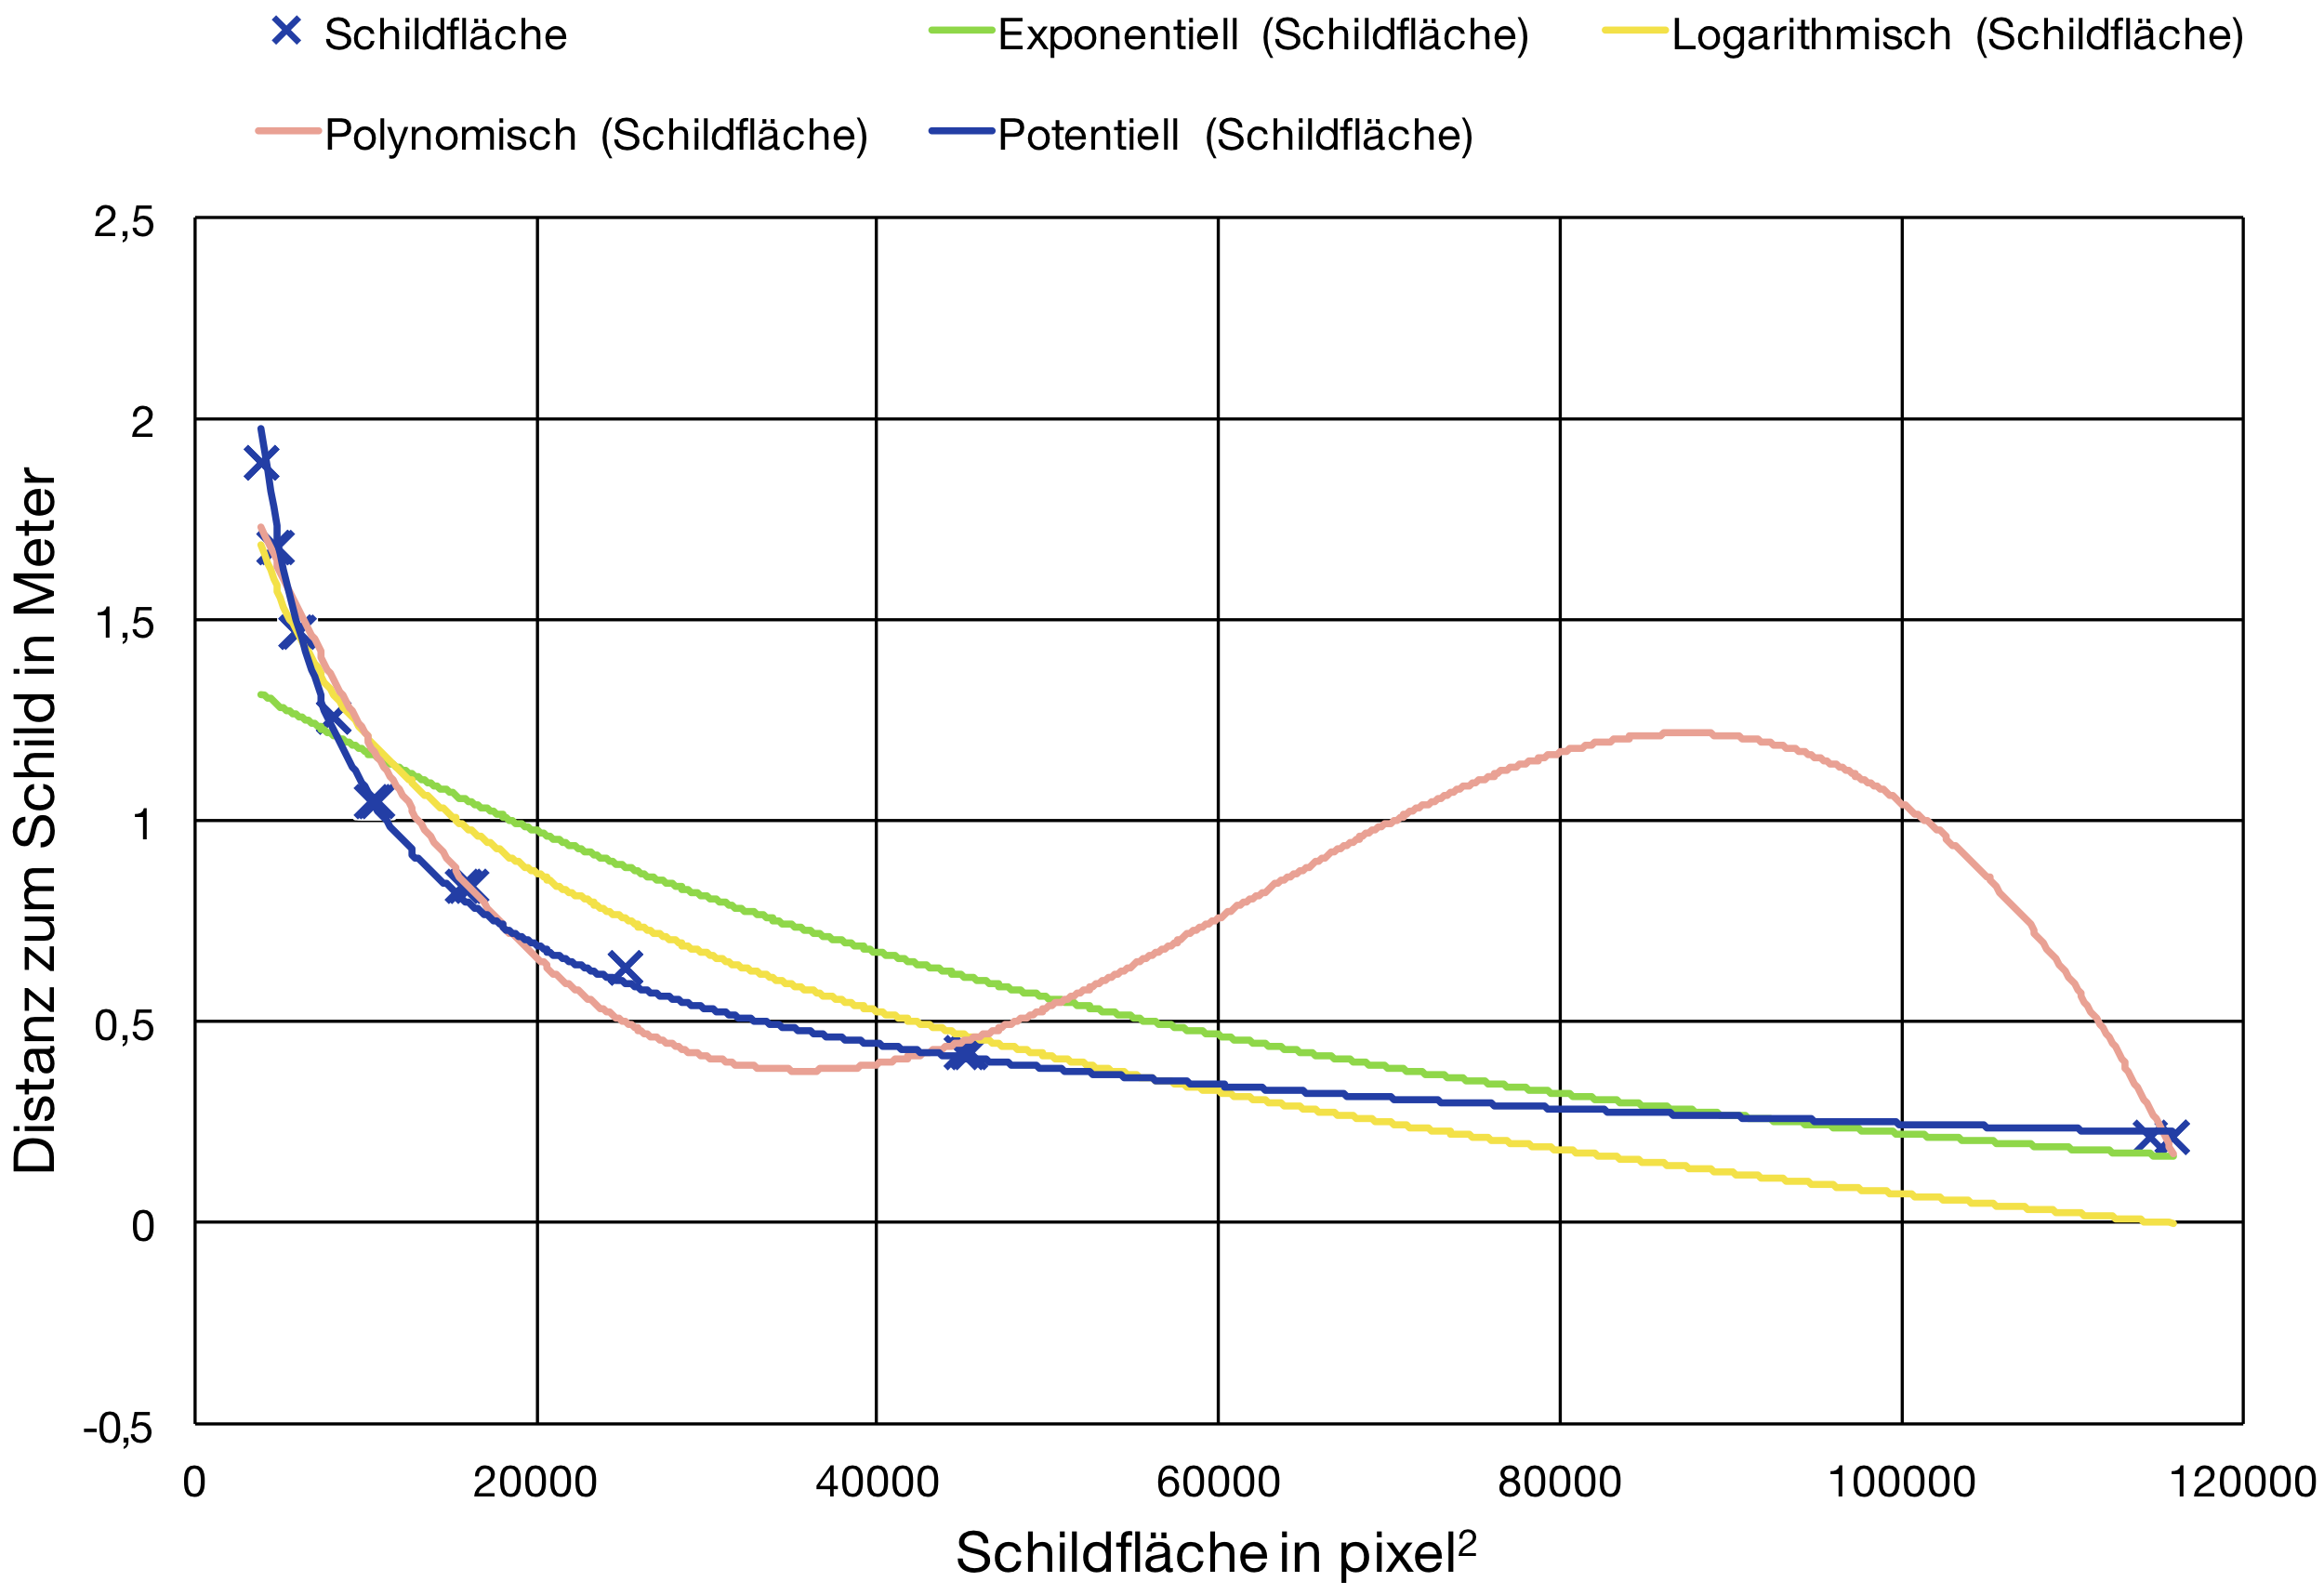
\includegraphics[width=0.8\textwidth]{pics/Schildererkennung_Distanz.png}
	\caption{Messpunkte f�r Verh�ltnis Fl�che zu Distanz und verschiedene Regressionsfunktionen}
	\label{fig:v4}
\end{figure}

\subsection{Ausblick: Verbesserungsm�glichkeiten}
Man kann �berlegen, einen anderen Deskriptor als SURF zu verwenden. Dieser ist zwar f�r Forschungszwecke lizenzfrei aber nicht f�r kommerzielle Zwecke. Wom�glich ist der lizenzfreie (BSD-Lizenz) Deskriptor ORB \cite{rublee2011orb} eine bessere L�sung.

Bei der aktuellen Implementierung werden jedes Mal, wenn ein neues Kamera-Bild verarbeitet wird, beim Referenzbild des Schildes von neuem die Keypoints gesucht. Da diese sich aber nicht ver�ndern, k�nnte man diesen Schritt auslagern, sodass er nur einmal ausgef�hrt wird.

Au�erdem k�nnte man die Schilderkennung erweitern, sodass mehr als nur drei Schilder erkannt werden.


	\clearpage
	\section{Auswertung}
	\clearpage
	\section{Konklusion}

Das Projektseminar stellte sich als eine sehr vielf�ltige und facettenreiche Veranstaltung heraus, bei der das eigentliche Ziel, eine Fahrzeugsteuerung zu programmieren, nur einen Teil der Erkenntnisse darstellt.

Durch den l�ngeren Zeitraum von einem Semester konnten wir uns intensiv mit Ans�tzen des Autonomen Fahrens besch�ftigen und konnten so mit Integrationstests und Projektplanung auf eine spannende und praxisnahe Art und Weise vieles lernen. Insbesondere die Einarbeitung und Verwendung verschiedener Tools in der Software-Entwicklungskette war besonders sinnvoll.

Auch war es sehr interessant, den Umgang mit der Roboter-Middleware ROS zu erlernen. Dass dieses System auch in der Industrie eingesetzt wird, zeigt die Wichtigkeit der F�higkeit, sich in neue Software-L�sungen einzuarbeiten.

Wir konnten auf eine sehr umfangreiche und freundliche Projektbetreuung zur�ckgreifen, sodass wir f�r die verschiedenen Probleme immer einen Ansprechpartner hatten. Sehr hervorzuheben ist auch die freie Gestaltung der Aufgaben. Der genaue Zeitplan war uns �berlassen, die Zusatzaufgabe durften wir uns selbst �berlegen.

Dennoch kamen wir auch mit unseren vergleichsweise primitiven Berechnungen an die Leistungsgrenzen der Recheneinheit. Hier w�re es n�tzlich, die Rechenleistung zu erh�hen, damit Bilder besser verarbeitet werden k�nnten. Auch sind bessere Lenk- und Fahrmotoren wichtig, um Performanzsteigerungen zu erreichen.

Insbesondere hinsichtlich des zuk�nftigen Ziels des Carolo-Cups bietet es sich an, die implementierten Module zu verbessern. Die Regelung l�sst noch viele weitere Verbesserungen zu, w�hrend die Schilderkennung weiter optimiert und erweitert werden kann.


	\clearpage
	
	\bibliographystyle{alphadin}
	\bibliography{literature}

\end{document}
